\subsection{Work}

The mathematical concept of work is an application of vectors in $\R^n$.  The physical concept
of work differs from the notion of work employed in
ordinary conversation. For example, suppose you were to slide an object of mass 150 kilograms
off a table which is one meter high and carry the object to another table 50 meters away, keeping the object always exactly one meter above ground. The physical concept
of work would indicate that the force exerted by your arms did no work
during this project. The reason for this definition is that even
though your arms exerted considerable force on the object, the direction of motion was at right angles to the force they
exerted. The only part of a force which does work in the sense of physics is
the component of the force in the direction of motion.

Work is defined to be the magnitude of the component of
this force times the distance over which it acts, when the 
component of force points in the direction of motion. In the case where the force points in exactly the opposite direction of motion
work is given by $\tup{-1} $
times the magnitude of this component times the distance.
Thus the work done by a force on an object as
the object moves from one point to another is a measure of the extent to
which the force contributes to the motion. This is illustrated in the
following picture in the case where the given force contributes to the
motion.

\begin{center}
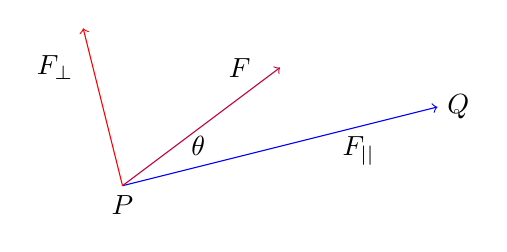
\begin{tikzpicture}
\draw[blue, ->](0,0)--(4,1);
\draw[purple, ->](0,0)--(2,1.5);
\draw[red, ->](0,0)--(-0.5, 2);
\node[below] at (0,0){$P$};
\node[right] at (4,1){$Q$};
\node[left] at (-0.5,1.5){$\vect{F}_{\perp}$};
\node[left] at (1.75,1.5){$\vect{F}$};
\node[below] at (3,0.75){$\vect{F}_{||}$};
\node[right] at (0.75, 0.5){$\theta$};
\end{tikzpicture}
\end{center}

Recall that for any vector $\vect{u}$ in $\R^n$, we can write $\vect{u}$ as a sum
of two vectors, as in
\begin{equation*}
\vect{u} = \vect{u}_{||} + \vect{u}_{\perp}
\end{equation*}
For any force $\vect{F}$,  
we can write this force as the sum of a vector in the direction of the motion and a vector
perpendicular to the motion. In other words,
\begin{equation*}
\vect{F} = \vect{F}_{||} + \vect{F}_{\bot}
\end{equation*}

In the above picture the force, $\vect{F}$ is applied to an object which moves
on the straight line from $P$ to $Q$. There are two vectors shown, $\vect{F}_{||}$ and $\vect{F}_{\bot }$ and the
picture is intended to indicate that when you add these two vectors you get 
$\vect{F}$. In other words, $\vect{F} = \vect{F}_{||} + \vect{F}_{\bot}$. Notice that
 $\vect{F}_{||}$ acts in the direction of motion and 
$\vect{F}_{\bot }$ acts perpendicular to the direction of motion. Only 
$\vect{F}_{||}$ contributes to the work done by $\vect{F}$ on the object
as it moves from $P$ to $Q$. $\vect{F}_{||}$ is
called the component of the force in
\index{component of a force} the direction of motion. From trigonometry, you
see the magnitude of $\vect{F}_{||}$ should equal $\norm{\vect{F}
} \abs{\cos \theta}$. Thus, since $\vect{F}_{||}$ points
in the direction of the vector from $P$ to $Q$,
the total work done should equal
\begin{equation*}
\norm{\vect{F}} \norm{
\longvect{PQ}} \cos \theta =\norm{
\vect{F}} \norm{\vect{q}-\vect{p}} \cos \theta
\end{equation*}

Now, suppose the included angle had been obtuse. Then the work done by the force 
$\vect{F}$ on the object would have been negative because $\vect{F}_{||}$
would point in $-1$ times the direction of the motion.  In this case, $\cos \theta $ would also be negative and 
so it is still
the case that the work done would be given by the above formula. Thus from
the geometric description of the dot product given above, the work equals
\begin{equation*}
\norm{\vect{F}} \norm{\vect{q}-\vect{p}} \cos
\theta =\vect{F}\dotprod \tup{\vect{q}-\vect{p}} 
\end{equation*}
This explains the following definition.

\begin{definition}{Work done on an object by a force}{work-done-by-force}
Let $\vect{F}$ be a force acting on an object which moves from the point 
$P$ to the point $Q$, which have position vectors given by $\vect{p}$ and $\vect{q}$ respectively.
 Then the \textbf{work} done
\index{work} on the object by the given force equals $\vect{F}\dotprod \tup{
\vect{q}-\vect{p}} $.
\end{definition}

Consider the following example.

\begin{example}{Finding work}{finding-work}
Let $\vect{F}=
\begin{mymatrix}{rrr}
2 & 7 & -3
\end{mymatrix}^T$ Newtons. Find the work
done by this force in moving from the point $\tup{1,2,3} $ to the
point $\tup{-9,-3,4} $ along the straight line segment joining these
points where distances are measured in meters.
\end{example}

\begin{solution}
First, compute the vector $\vect{q} - \vect{p}$, given by 
\begin{equation*}
\begin{mymatrix}{rrr}
-9 & -3 & 4
\end{mymatrix}^T
-
\begin{mymatrix}{rrr}
1 & 2 & 3
\end{mymatrix}^T
=
\begin{mymatrix}{rrr}
-10 & -5 & 1
\end{mymatrix}^T
\end{equation*}

According to Definition \ref{def:work-done-by-force} the work done is
\begin{align*}
\begin{mymatrix}{rrr}
2 & 7 & 3
\end{mymatrix}^T
 \dotprod 
\begin{mymatrix}{rrr}
-10 & -5 & 1
\end{mymatrix}^T
& =-20+\tup{-35} +\tup{
-3} \\
& =-58\text{ Newton meters}
\end{align*}
\end{solution}

Note that if the force had been given in pounds and the distance had been
given in feet, the units on the work would have been foot pounds. In
general, work has units equal to units of a force times units of a length.
Recall that $1$ Newton meter is equal to $1$ Joule.  Also notice that the work done by the force can be negative as in the
above example.
